\newpage
\section{Veracity真實度模型}
現今大數據的興起,資料科學也是風行全球。然而在做資料分析的時候,大家最關心的是資料的可性度,也就是大數據5V當中的Veracity。而建構在資料理解性上的真實度時,因為每一個人在看資料的時候,所看的面向是不同的,所以這就造成的標準不同。所以本研究提出Veracity 真實度模型來提出一個量化的方式解決這個問題。
\subsection{模型理論}
真實度模型是建構在資料理解性(data understandability)上,而所謂的資料理解性不像一般常見的對於XML文件相似度的比較。例如要說這兩份資料的真實度很高,也許大家從不同角度觀察,結果都不盡相同。這樣評量資料真實度就顯得很抽象,本研究即提供一個量化的方式,也就是真實度模型來針對XML做分數量化,讓使用者自行設計量化方法,來決定如何把抽象化為具體的評比分數。\\\par

而在真實度模型(Veracity Model)的架構之下會有多個維度(Dimension),在維度之下會有的多個屬性(Attribute ),每一個屬性之下都有其量化的方法(Quantification)。假設有一份基準XML文件B(Base XML Document)以及被量測文件M(Measure XML Document),而文件M將被量測與文件B的真實程度(Veracity Value)。這樣就可以計算出文件M在真實度模型中的真實分數。而每一個維度也可以根據下面所屬的屬性計算出維度的分數(Dimension Degree),也可以得到維度下方每一個屬性的分數(Score)。\\\par

真實度模型($M$)的架構當中,會有多個真實維度來表示使用者理解資料的多個面向。每一個維度會描述使用者對於資料理解性的每一個面向。下面定義了一個模型有n個維度,$D_i$表示模型當中的第n個維度:
$$
M=\{D_i\}\ ,\ i= 1\ to\ n
$$
在真實維度$D_i$當中會有多個真實屬性來描述真實維度的細節。舉例來說,使用者認為資料來源可視為一個維度,那麼這個維度的屬性可能會有來源網址、文件編碼等等,這樣可以定義成真實維度$D_i$當中的$A_{i,j}$個屬性:
$$
D_i=\{A_{i,j}\}\ ,\ j=1\ to\ n
$$
在真實屬性$A_{i,j}$當中,會有其量化的方法$Q_{i,j}$。讓使用者可以針對每一項屬性去描述如何量化以及在量化的時候可能需要做的正規化。\\\par

綜合以上,我們可以從每一個維度的真實屬性中的量化方式得到屬性的分數。且根據不同屬性做權重$w_{i,j}$的調整,再自定義函數$F_A()$來計算所有屬性與權重,進而得到維度的分數:
$$
\left\lvert D_{i}\right\rvert=F_A(w_{i,j},\  \left\lvert Q_{i, j}\right\lvert)
$$
%整個真實度模型的估算方式Fd
而從上述所得到的維度分數與權重$W_{i}$做調整,並且放入自定義函數$F_D()$中即可得到整體真實度模型的分數:
$$
 \left\lvert M\right\lvert=F_D(W_i,\ \left\lvert D_{i}\right\lvert)
$$

\subsection{UML表達方式}
基於上述理論模型,使用UML建構模型之物件導向關係圖。真實度模型使用UML來表示如圖\ref{uml}所示。在圖\ref{uml}當中有Model、Dimension和 Attribute這三個抽象類別。在設計的時候,每一個類別都必須繼承這三個類別的其中一個,並且實作內容。實做出來的子類別則會產生組合的關係。如Model下面會有多個Dimension;Dimension下則會有多個Attribute,且三個類別互相相依,當Dimension下沒有Attribute的時候,這個Dimension將不存在;而當Model 下沒有Dimension,則這個Model也不存在。

\begin{figure}[H]
\centering
\graphicspath{{/Users/FUDA/Documents/masterThesis/image/}}
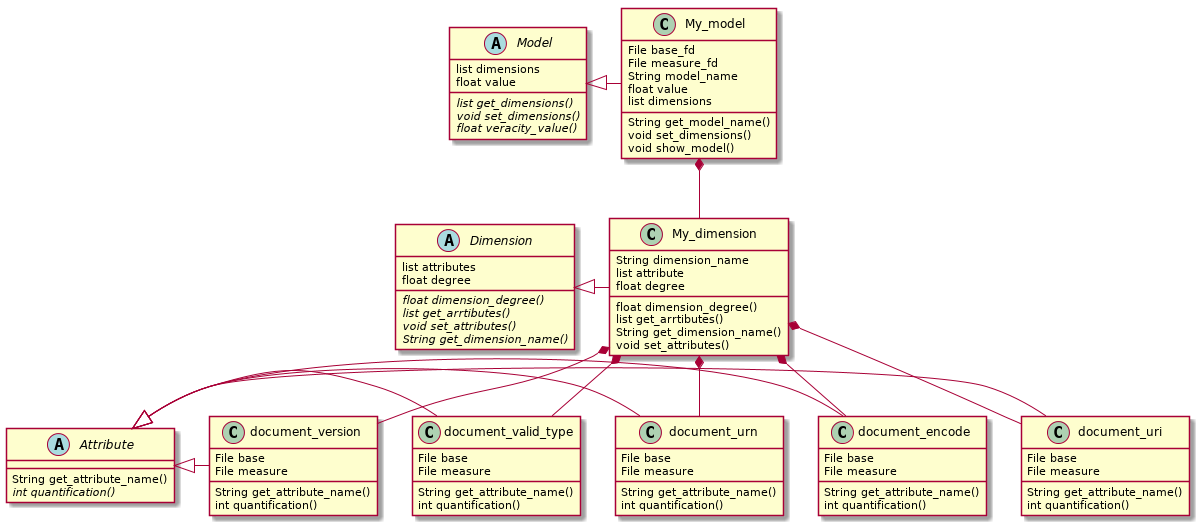
\includegraphics[scale=0.42]{uml.png}
\caption{真實度模型}
\label{uml}
\end{figure}

上述之UML提供一個物件導向的程式架構,把前面的理論模型轉換為可程式化的方法。也就是只要有這樣的模型以及敘述,使用任一種程式語言皆可以實作本研究之模型,進而達到使用者在選擇程式語言實現本模型時候的彈性。\\\par

在實現本模型的時候,需要注意的是抽象類別的繼承與改寫以及物件的組合關係。首先是抽象類別的繼承與改寫,使用者須繼承抽象類別並進行實作。假設進行了繼承卻沒有實作,那麼程式將無法正常動作。再來是物件的組合關係,前面說到三個類別是具有相依關係的。也就是在實作的時候,每一個Dimension下至少要有一個Attribute,這樣這個Dimension才得以存在。而每一個Model下至少要有一個Dimension,這樣Model才算成立。

\subsection{應用範例}
如果手上有如氣象局資料,資料節錄如圖\ref{applicationexample}所示,希望可以鑑別手上資料真實度,那真實度模型可以依照使用者不同的需求自定義真實度屬性,例如使用者從基準文件觀察到氣象局的XML有一些特殊術語,所以可將一個維度設定為tag名稱比對。還有樹狀結構的路徑、tag數量、樹的深度等。定義好屬性後即可以定義維度,例如將有關結構的屬性歸類為一個維度,有關文件內容的屬性歸類為一個維度。這樣模型可以使用樹狀結構表示,如圖\ref{modelexample}所示:
\begin{figure}[H]
\centering
\graphicspath{{/Users/FUDA/Documents/masterThesis/image/}}
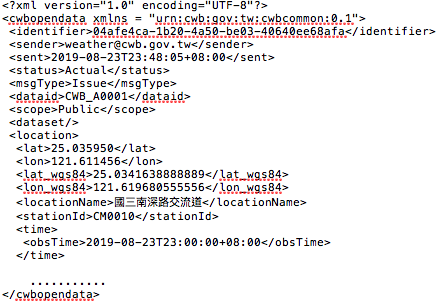
\includegraphics[scale=0.8]{weatherapplication.png}
\caption{氣象局資料節錄}
\label{applicationexample}
\end{figure}

\begin{figure}[H]
\centering
\graphicspath{{/Users/FUDA/Documents/masterThesis/image/}}
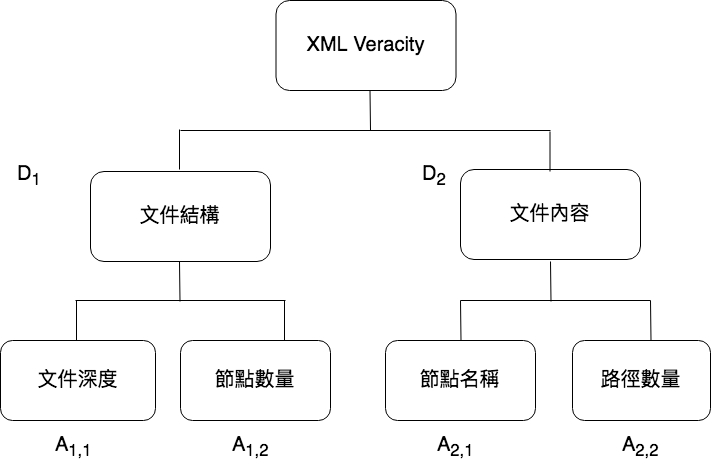
\includegraphics[scale=0.5]{modelexample.png}
\caption{真實度模型樹狀圖}
\label{modelexample}
\end{figure}

有了這樣的樹狀結構,即可以依照這樣的結構再加上前述的UML以及模型理論,即可以建構出符合資料特性的真實模型。\\\par
而在圖\ref{modelexample}當中,設計有兩個維度,兩個屬性的模型。首先在模型當中定義有兩個維度:
$$
M=\{D_1,\ D_2\}\\
$$
維度$D_1$代表樹狀圖上的文件結構,當中有$A_{1,1}$文件深度以及$A_{1,2}$節點數量兩個屬性,所以整個維度的定義如下:
$$
D_1=\{A_{1,1},\ A_{1,2}\}\\
$$

維度$D_2$代表樹狀結構上的文件內容,當中有$A_{2,1}$節點名稱以及$A_{2,2}$路徑數量兩個屬性,維度$D_2$的定義如下
$$
D_2=\{A_{1,1},\ A_{1,2}\}\\
$$
接著可以決定各個屬性的量化方法(Quantification),文件深度的部分,文件深度的部分可以與基準文件進行比較,如果層數只有相差5層以內或一定比例以內,可以進行一定比例的加減分或給予滿分,這樣即可以得到$Q_{1,1}$,而計分公式則可以這樣表示:
$$
Q_{1,1}=100-(10\times (\left\lvert BaseFileDepth-MeasureFileDepth\right\lvert)
$$
節點數量方面會跟基準文件的節點數量比較過後看相差多少,如數量上相差不大,分數也可以斟酌給分,若差異過大則可以考慮依比例倒扣分數。這樣可以得到$Q_{1,2}$。計分公式表示如下:
$$
Q_{1,2}=100\times (1-(0.02 \times (\left\lvert BaseFileTagCount-MeasureFileTagCOUNT\right\lvert)))
$$
文件內容的部分,在節點名稱的屬性中,可以比較與基準文件的節點名稱命名,可以隨機挑選數個節點出來做比較,再依照被量測文件是否有包含挑選出的節點,來依照比例給分。即可以得到$Q_{2,1}$,$Q_{2,1}$公式定義如下:
$$
Q_{2,1}=100\times \frac{MatchTag}{BaseFileTag}
$$
路徑數量中可以去計算基準文件有幾條路徑,被量測文件跟基準文件相差多少,再依照比例加減分,即可得到$Q_{2,2}$,$Q_{2,2}$的定義如下:
$$
Q_{2,2}=100-(10\times (\left\lvert BaseFilePath-MeasureFilePath\right\lvert)
$$
屬性的量化方式決定完成後,維度的量化方式$F_A()$可以定義為加總來得到,公式如下:
$$
D_i=\sum_{j=1}^{2} Q_{i,j}
$$
模型的最後真實度評分也是透過將維度的分數加總來得到,公式定義如下,這樣即完成了真實度的評比及量化。
 $$
 M=\sum_{i=1}^{2} D_i
 $$
